\documentclass[aspectratio=169]{beamer}

\usetheme{boxes}
\useinnertheme{circles}

\definecolor{UC}{RGB}{0, 50, 98}
\definecolor{Beamer}{RGB}{51, 51, 178}
\definecolor{Hooker}{RGB}{73, 121, 107}
\definecolor{Triton}{RGB}{0, 106, 150}
\definecolor{Prussian}{RGB}{0, 49, 83}
\definecolor{Forest}{RGB}{101, 121, 48}
\definecolor{Metro}{RGB}{35, 55, 59}
\definecolor{Gamboge}{RGB}{228, 155, 15}
\definecolor{Devil}{RGB}{115, 39, 43}
\definecolor{Shade}{RGB}{250, 250, 250}
\definecolor{JPAL}{RGB}{227, 89, 37}
\definecolor{IPA}{RGB}{90, 128, 38}

\usecolortheme[named=Triton]{structure}

% \setbeamercolor{background canvas}{bg=Shade}
\setbeamercolor{block title}{bg=Beamer!12}
\setbeamercolor{block body}{bg=Beamer!8}

\setbeamersize{text margin left=0.2in,text margin right=0.2in}

% \setbeamertemplate{footline} % To remove the footer line in all slides uncomment this line
\setbeamertemplate{footline}[page number] % To replace the footer line in all slides with a simple slide count uncomment this line
\setbeamertemplate{navigation symbols}{} % To remove the navigation symbols from the bottom of all slides uncomment this line
\setbeamertemplate{bibliography item}{}
\setbeamertemplate{caption}[numbered]

\setbeamertemplate{frametitle}{%
    \usebeamerfont{frametitle} \vspace{0.5em} \insertframetitle%
    \vphantom{g}% To avoid fluctuations per frame
    \vspace{0.5em} \hrule% Uncomment to see desired effect, without a full-width hrule
    \par\hspace*{-\dimexpr0.5\textwidth-0.5\textwidth}\rule[0.5\baselineskip]{\textwidth}{0.4pt}
    \par\vspace*{-\baselineskip}% <-- reduce vertical space after rule
}

\usepackage[T1]{fontenc}
\usepackage{inconsolata}
\usepackage[sfdefault,light]{roboto}
% \usepackage[sfdefault,light]{FiraSans}
\usepackage{amsmath, amssymb, amsthm, mathrsfs, bbm}
\usepackage{threeparttable, adjustbox, tabularx, booktabs}
\usepackage{appendixnumberbeamer}
\usepackage{hyperref}
\usepackage{pdflscape}
\usepackage{placeins}
\usepackage{caption}
\usepackage{graphicx}
\usepackage{listings}
\usepackage{color}
\usepackage{tfrupee}
\usepackage[backend=bibtex, style=authortitle, citestyle=authoryear-icomp, url=false]{biblatex}
\addbibresource{Lottery.bib}

\newcommand{\inv}[1]{#1^{-1}}
\newcommand{\iid}{\text{i.i.d.}}
\newcommand{\bmat}[1]{\begin{bmatrix} #1 \end{bmatrix}}
\newcommand{\asconv}{\xrightarrow{a.s.}}
\newcommand{\pconv}{\xrightarrow{p}}
\newcommand{\dconv}{\xrightarrow{d}}
\newcommand{\msconv}{\xrightarrow{m.s.}}
\newcommand{\liminfty}{\lim_{n \to \infty}}
\newcommand*\diff{\mathop{}\!\text{d}}
\newcommand{\lhood}{\mathcal{L}}
\newcommand{\var}{\text{Var}}
\newcommand{\ev}{\text{E}}
\renewcommand{\vec}[1]{\mathbf{#1}}
\newcommand{\specialcell}[2][c]{\begin{tabular}[#1]{@{}c@{}}#2\end{tabular}}

\newtheorem{prop}{Proposition}
\newtheorem{claim}{Claim}
\newtheorem{assume}{Assumption}
\newtheorem{define}{Definition}

\newenvironment{wideitemize}{\itemize\addtolength{\itemsep}{10pt}}{\enditemize}
\newenvironment{wideenumerate}{\enumerate\addtolength{\itemsep}{10pt}}{\endenumerate}

\let\oldforall\forall
\let\forall\undefined
\DeclareMathOperator{\forall}{\oldforall}
\DeclareMathOperator*{\argmax}{arg\,max}
\DeclareMathOperator*{\argmin}{arg\,min}

\lstset{
  basicstyle=\footnotesize\ttfamily,
  columns=fixed,
  fontadjust=true,
  basewidth=0.5em
}

\title{Regret Aversion in Prize-Linked Savings: Evidence From Kenya}
\author[Abraham]{Justin Abraham}
\institute{University of California, San Diego}
\date{\today}

\begin{document}

\begin{frame}
	\titlepage
\end{frame}

\begin{frame}{Motivation}

	\begin{wideitemize}

		\item One behavioral approach: build decision theoretic models that reflect psychological processes.

		\item There is strong evidence that regret is an important factor in our decision making.

		\item Preferences incorporating regret aversion have been used to rationalize Allais and explain why (risk-averse) individuals play lotteries.

	\end{wideitemize}

\end{frame}

\begin{frame}{Motivation}

	\begin{block}{Regret}
	 ``...a negative, cognitively based emotion that we experience when realizing or imagining that our present situation would have been better, had we decided differently.''
	\end{block}

	Preferences depend on comparison between realized outcomes and foregone outcomes \parencite{bell_risk_1983,loomes_regret_1982}. 

	\[ EU(f | f, g \in B) =  \sum_i p_{i} \cdot Q\left(u\left(f_{i}\right)-u\left(g_{i}\right)\right) \]
	
\end{frame}

\begin{frame}{Research Question}

	\begin{wideitemize}

		\item Does regret aversion induce greater participation in prize-linked savings? (Yes)
		\item How does the effect of regret aversion change over time?

			\begin{wideenumerate}
				\item Repeated experience can make the feeling of regret more salient.
				\item Regret aversion may have diminishing sensitivity.
			\end{wideenumerate}

	\end{wideitemize}

\end{frame}

\begin{frame}{Overview}

	\begin{wideenumerate}

		\item Use experimental data from a savings experiment conducted in Nairobi.
		\item Estimate a one-shot model of regret aversion using first period data in a calibration exercise.
		\item Propose a model of dynamic regret aversion.
		\item Test for decreasing/increasing effects over time.

	\end{wideenumerate}

\end{frame}

\begin{frame}{Data}

	\begin{itemize}
	\item 311 respondents from informal settlements in Nairobi
		\begin{enumerate}
		\item Matched incentives account (105)
		\item Lottery-linked account (103)
		\item Lottery-linked account with regret (103)
		\end{enumerate}
	\item Lab component at baseline
		\begin{enumerate}
		\item Risk aversion 
		\item Temporal discounting
		\item Willingness-to-pay to play a lottery
		\item Internal locus of control
		\item Gambling questionnaire
		\item Demographics questionnaire
		\end{enumerate}
	\item Observed transactions over a 60-day period
	\item Endline questionnaire
	\end{itemize}

	% Nearly 60% of our sample is female with a median age of 28 years.Less than half of the participants in our sample reported that they are employedwith only 5% reported receiving a regular income. The median PPP-adjustedmonthly income among those employed is USD 77.2Approximately 55% ofour sample saves regularly with a majority of savers utilizing rotating savingsand credit associations (ROSCA), a type of informal group savings.  Averagemonthly savings among these individuals amount to USD 23. A small fractionof the sample save with M-Shwari, a mobile banking service offering a basicpaperless account and access to credit. Transactions are made with M-Pesa, anSMS-based money system made accessible by the ubiquity of mobile phones inKenya.

\end{frame}

\begin{frame}{Experiment}

	\begin{block}{Matching}
		\begin{itemize}
		\item Fixed 5\% match on daily deposits
		\item Contributions dispayed at end of day
		\end{itemize}
	\end{block}

	\begin{block}{Lottery}
		\begin{itemize}
		\item Entered into a daily lottery if saved a non-zero amount
		\item Prize equal in expectation to 5\% match
		\end{itemize}
	\end{block}

	\begin{block}{Lottery with Feedback}
		\begin{itemize}
		\item Payoffs identical to lottery group
		\item \textbf{Lottery outcomes provided every morning regardless of deposit}
		\end{itemize}
	\end{block}

\end{frame}

\begin{frame}{Preliminary Results}

	\begin{figure}[H]
		\centering
		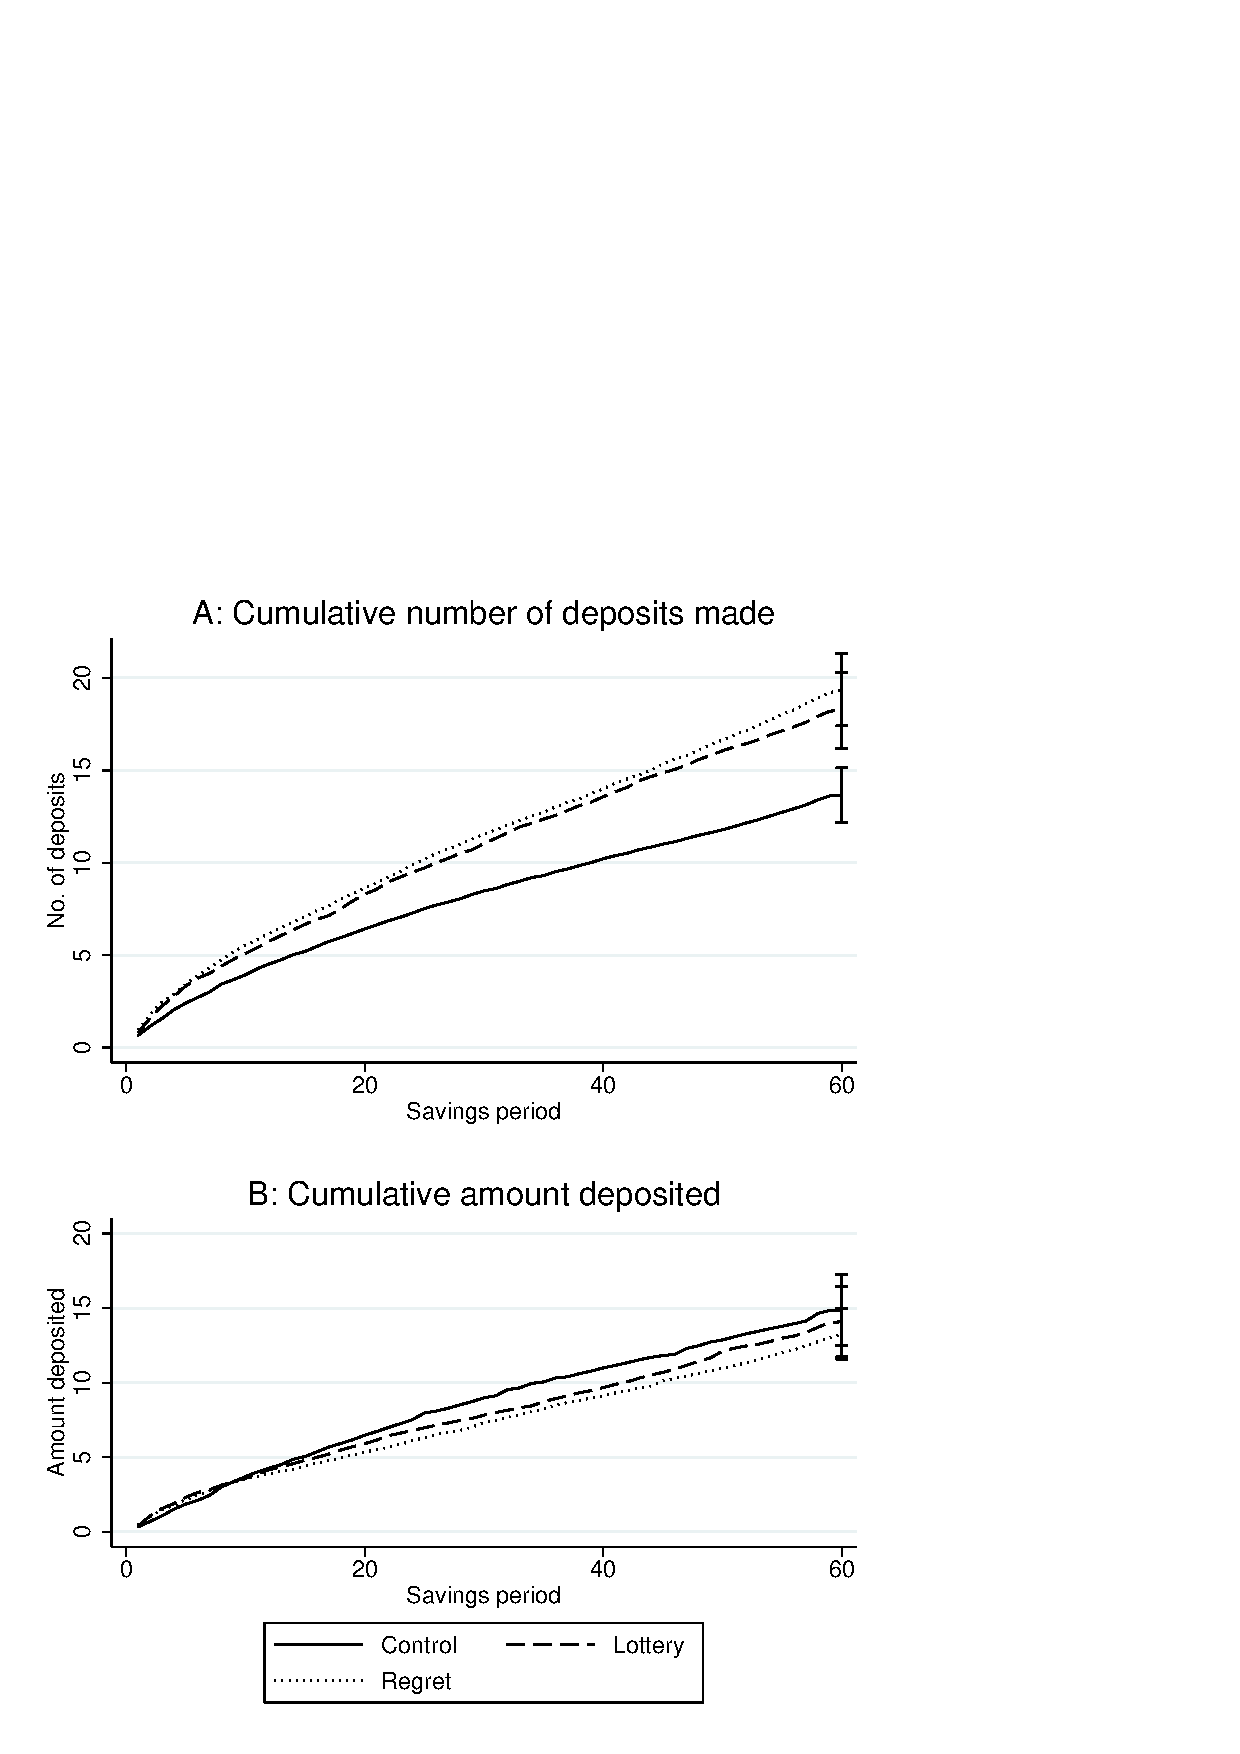
\includegraphics[width=0.35\linewidth]{line-cumdeposits.pdf}
	\end{figure}

\end{frame}

\begin{frame}{Preliminary Results}

	\begin{figure}[H]
		\centering
		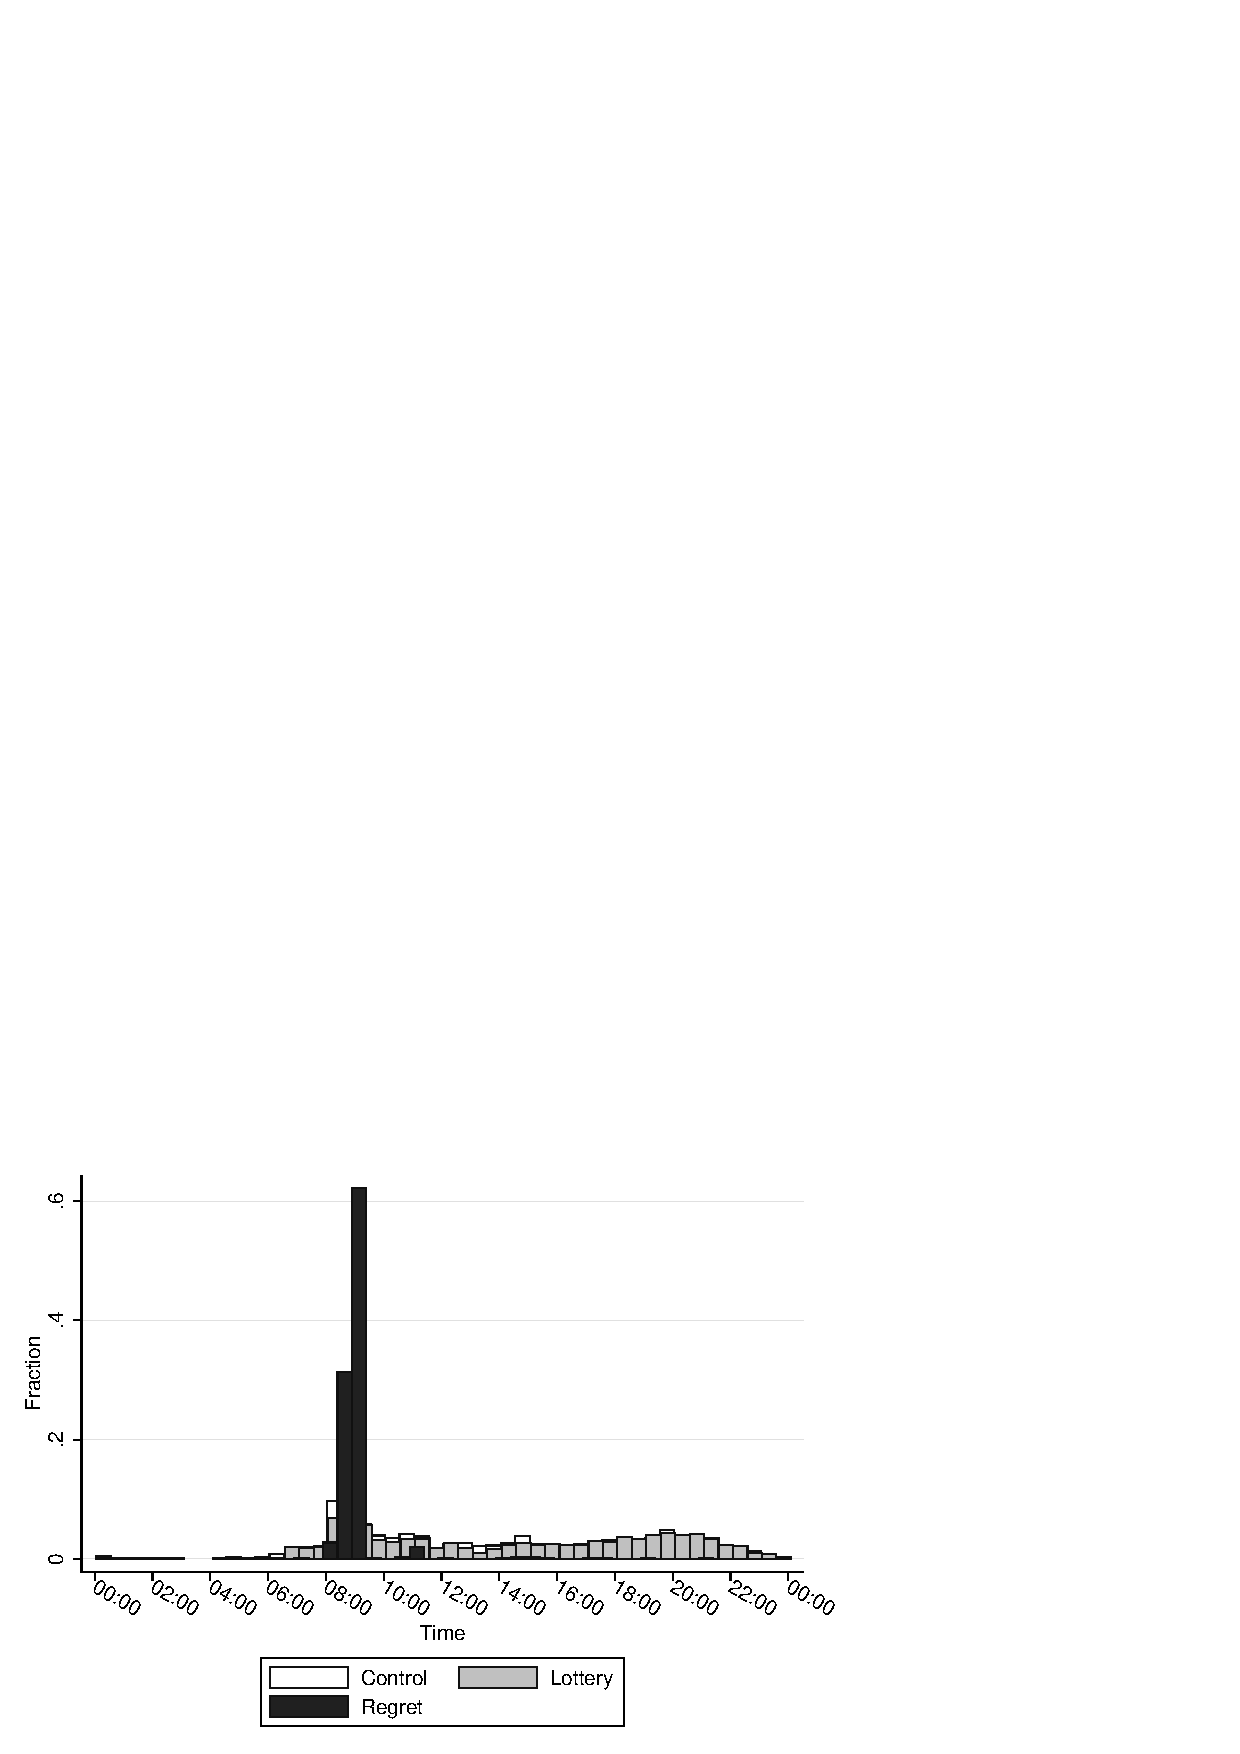
\includegraphics[width=0.65\linewidth]{hist-deposits.pdf}
	\end{figure}

\end{frame}

\begin{frame}{Literature}

	\begin{wideenumerate}

		\item Lottery incentives motivate individuals over non-stochastic incentives \parencite{herskowitz_gambling_2016,atalay_savings_2014,filiz-ozbay_lottery_2015,cookson_when_2016,dizon_leveraging_2016}.
		\item ``Behaviorally-informed'' savings technologies in developing countries \parencite{akbas_how_2016,karlan_getting_2010,thaler_save_2004,ashraf_tying_2006,dupas_why_2013}. 
		\item Empirical tests of regret aversion using feedback manipulation \parencite{zeelenberg_consequences_1996,zeelenberg_consequences_2004,filiz-ozbay_auctions_2007}.
		\item How is this different from reference-dependent preferences? Maybe not.

	\end{wideenumerate}

\end{frame}

\begin{frame}[allowframebreaks] \frametitle{References}

	\printbibliography

\end{frame}

\end{document}